\documentclass[10pt,mathserif]{beamer}

\usepackage{graphicx,amsmath,amssymb,tikz,psfrag,subfigure,bm}

\input defs.tex

%% formatting

\mode<presentation>
{
\usetheme{default}
}
\setbeamertemplate{navigation symbols}{}
\usecolortheme[rgb={0,0,0}]{structure}
\setbeamertemplate{itemize subitem}{--}
\setbeamertemplate{frametitle} {
	\begin{center}
	  {\large\bf \insertframetitle}
	\end{center}
}

\AtBeginSection[] 
{ 
	\begin{frame}<beamer> 
		\frametitle{Outline} 
		\tableofcontents[currentsection,currentsubsection] 
	\end{frame} 
} 

%% begin presentation

\title{\large \bfseries Monte Carlo inference}

\author{Jiali Lin\\[3ex]
Virginia Tech}

\date{\today}

\begin{document}

\frame{
\thispagestyle{empty}
\titlepage
}

\section{Introduction}
\begin{frame}{Introduction}
\begin{itemize}
    \item We typically can draw sample $\bm{x}^s \overset{i.i.d}{\sim}f(\bm{x})$. 
    \item Now, we are unable to have this step.
    \item \textbf{Idea:} based on non-iterative algorithms of \textbf{Monte Carlo approximation}.
    \begin{itemize}
        \item Generate some (unweighted) samples from the posterior, $\bm{x}^s\sim p(\bm{x}|\mathcal{D})$ (where $s$ means ``sample").
        \item Use these to compute any quantity of interest, such as a posterior marginal, $p(x_1 - x_2|\mathcal{D})$.
    \end{itemize}
    \item Useful when we have complicated posterior distribution. 
\end{itemize}    
\end{frame}

\section{Sampling from inverse cdf}
\begin{frame}{Sampling from inverse cdf} 
\begin{itemize}
    \item Let $F$ be a cdf of target distribution and $F^{-1}$ be its inverse.
    \item We can sample from any univariate distribution, by evaluating its inverse cdf.
    \item Let $u$ represent the height up the $y$ axis. $u \sim U(0,1)$ using a pseudo random number generator.
    \item  \textbf{Idea:} ``slide along" the $x$ axis until intersecting the $F$ curve, ``drop down" to  return the corresponding $x$.
    \item  \textbf{Problems}: impossible to derive cdf $F(x)$.
\end{itemize}

\begin{figure}[h]
\centering
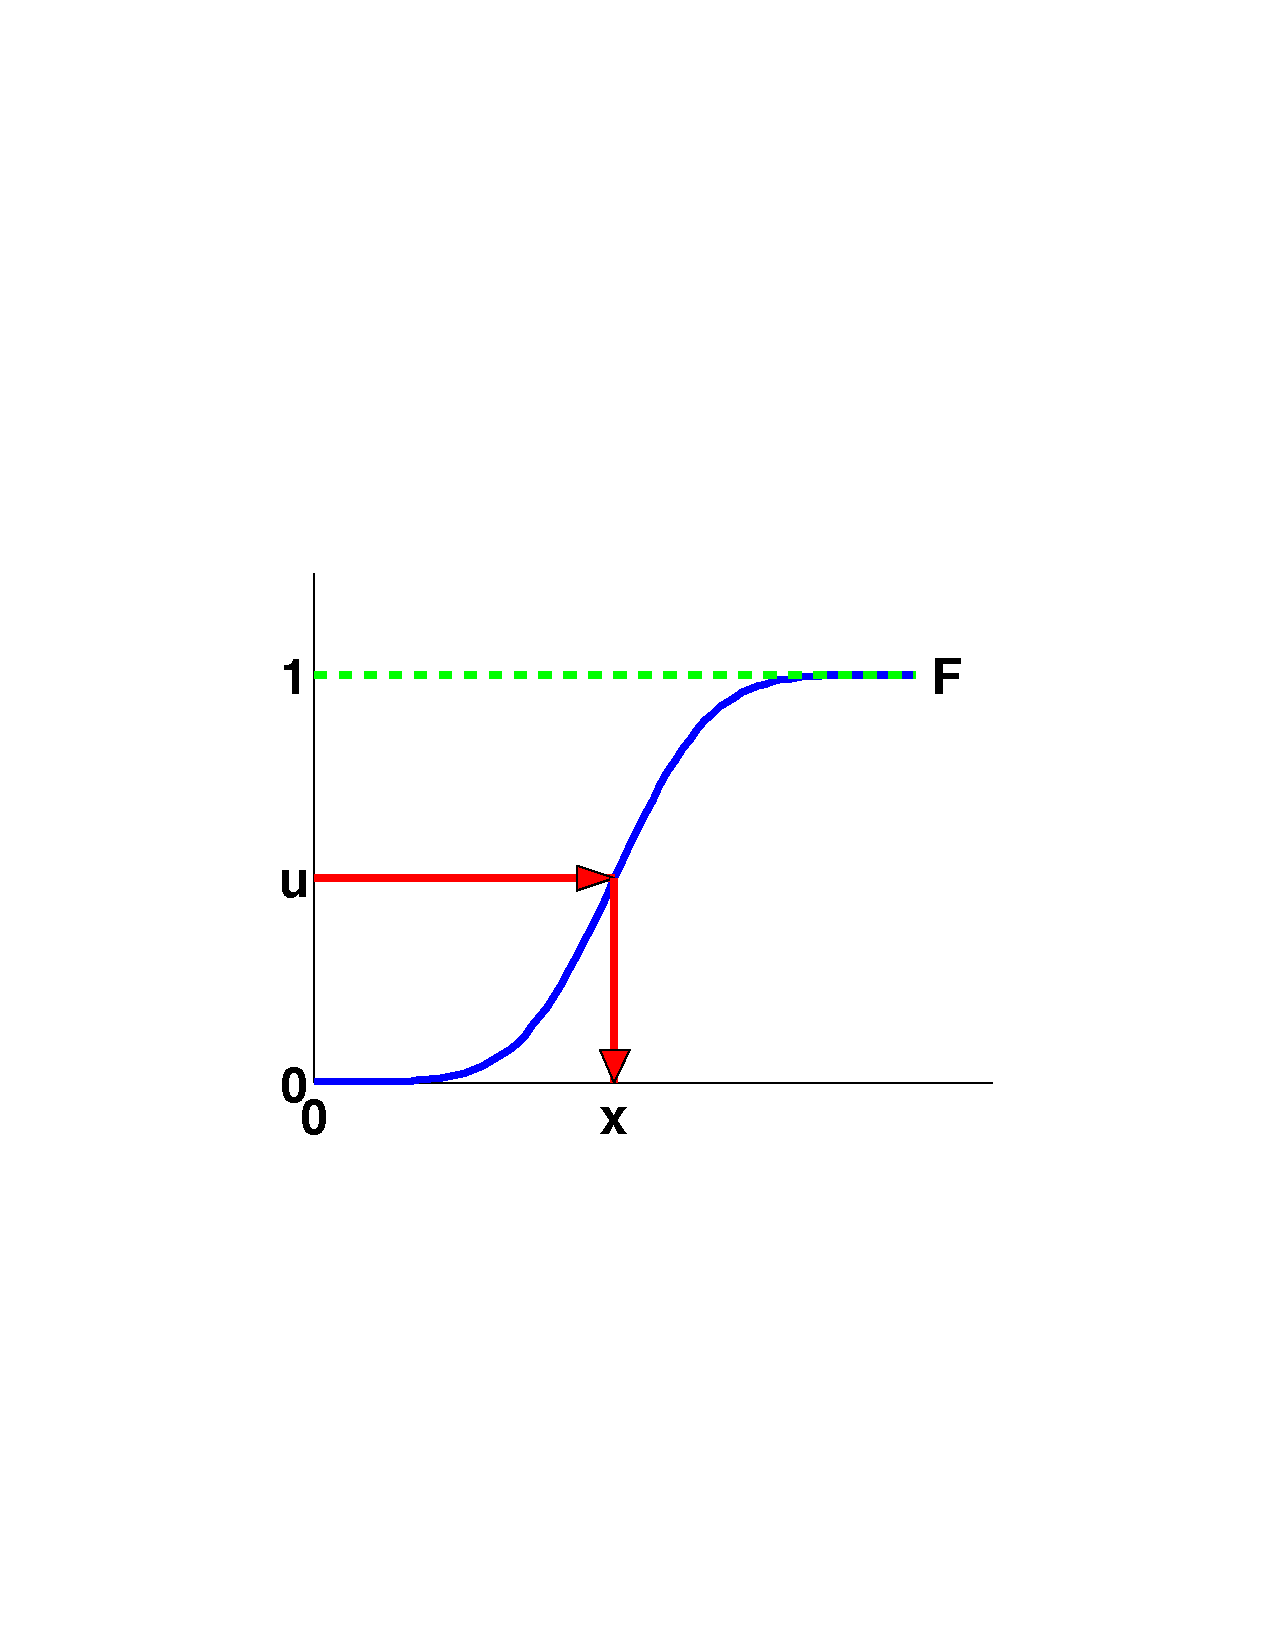
\includegraphics[width=0.3\textwidth]{sampleCdf}
\caption{Sampling using an inverse CDF. Figure generated by \texttt{CdfSamplingDemo}.}
\end{figure}    
\end{frame}

\section{Rejection sampling}
\begin{frame}{Rejection sampling}
\begin{itemize}
    \item \textbf{Goal:} reject samples from $q(x)$ such that they are sampled from $p(x)$.
    \item $q(x)$ must ``cover" or envelop the distribution $p(x)$ (i.e. $cq(x) > p(x)$ for all $x$).
    \item The samples are accepted if $\frac{p(x)}{cq(x)} > u $ where $u \sim Unif(0,1)$, and rejected otherwise.
    \item If the ratio is close to one, then $p(x)$ must have a large amount of probability mass around $x$ and that sample should be more likely accepted.
    \item If the ratio is small, then it means that $p(x)$ has low probability mass around $x$ and we should be less likely to accept the sample.
\end{itemize}    
\end{frame}

\begin{frame}{Illustration of rejection sampling}
\begin{figure}[h]
\centering
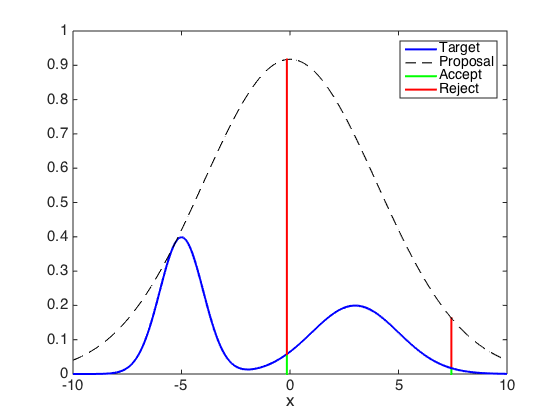
\includegraphics[width=0.5\textwidth]{rejectionSampling}
\caption{Rejection sampling from a mixture of two normal distributions using a proposal of normal distribution, where $c = \texttt{max(f(x)./q(x))}$. Figure generated by \texttt{R ejectionSampling}.}
\end{figure} 

\textbf{Comments:}
\begin{itemize}
    \item Hard to define proposal $q(x)$ before we know $p(x)$.
    \item $q(x)$ has to be closer to $p(x)$. Otherwise, it would be bad efficiency (low acceptance ratio).
    \item Fails in high dimensional space.
\end{itemize}
\end{frame}

\section{Importance sampling}
\begin{frame}{Importance sampling}
\begin{itemize}
    \item We can evaluate $p(\bm{x})$ easily for any given value of $\bm{x}$. 
    \item Proposal distribution $q(\bm{x})$ is easy to draw samples.
    \item \textbf{Ideas:} uses these samples to estimate the integral
    \begin{equation*} 
        I = E[f] = \int f(\bm{x})\frac{p(\bm{x})}{q(\bm{x})}q(\bm{x}) d\bm{x} \approx \frac{1}{S}\sum_{s=1}^S w_s f(\bm{x}^s)=\hat{I}
    \end{equation*} 
    where $w_s = \frac{p(\bm{x}^s)}{q(\bm{x}^s)}$ are the importance weights that can be computed.
    \item  Weights correct the bias introduced by sampling from the wrong distribution.
    \item Unlike rejection sampling, \textit{all the samples are used and focused on the important parts of space}.
    \item The latent sequence, $\bm{x}_{1:t}$ is determined by weight $\bm{w}_{1:t}$.
\end{itemize}    
\end{frame}

\begin{frame}{Importance sampling (cont'd)}
\begin{itemize}
    \item Usually $p(\bm{x}) =  \tilde{p}(\bm{x})/Z_p$, where $p(\bm{x})$ can be evaluated easily, whereas $Z_p$ is unknown. Then
    \begin{equation*} 
        E[f] = \frac{Z_q}{Z_p}\int f(\bm{x})\frac{\tilde{p}(\bm{x})}{\tilde{q}(\bm{x})}q(\bm{x}) d\bm{x} \approx \frac{Z_q}{Z_p}\frac{1}{S}\sum_{s=1}^S \tilde{w}_s f(\bm{x}^s)
    \end{equation*} 
    where $\tilde{w}_s = \frac{\tilde{p}(\bm{x}^s)}{\tilde{q}(\bm{x}^s)}$ is the unormalized importance weight.
    \item We can use the same set of samples to evaluate the ratio
    \begin{equation*} 
        \frac{Z_p}{Z_q} = \frac{1}{Z_p}\int\tilde{p}(\bm{x})d\bm{x} = \int\frac{\tilde{p}(\bm{x})}{\tilde{q}(\bm{x})} \approx \frac{1}{S}\sum_{s=1}^S \tilde{w}_s
    \end{equation*} 
    \item Hence
    \begin{equation*} 
        \hat{I} = \frac{\frac{1}{S}\sum_s \tilde{w}_s f(\bm{x}^s)}{\frac{1}{S}\sum_s \tilde{w}_s} =  \sum_{s = 1}^S w_s f(\bm{x}^s)
    \end{equation*} 
    where
    \begin{equation*} 
        w_s = \frac{\tilde{w}_s}{\sum_s' \tilde{w}_{s'}}
    \end{equation*} 
\end{itemize}    
\end{frame}

\section{Particle filtering}

\begin{frame}{Linear (Gaussian) State Space Models}
\begin{itemize}
    \item HMM structure with Gaussian conditional distributions:
    \begin{equation*}
        \begin{split}
            p(z_1) & =  N(z_1|0,Q_0)\\
            z_{t+1} & = Az_t + w_t, \quad w_t\sim N(0,Q)\\
            x_t & = Wz_t + v_t, \quad N(0,R)
        \end{split}
    \end{equation*}
    \item Hidden states and observations are jointly Gaussian, so all marginals are Gaussian (parameterized by mean \& covariance)/
    \item Posterior distribution of state at any time, given observations at any subset of other times, is Gaussian.
\end{itemize}
\end{frame}

\begin{frame}{Particle filtering}
\begin{itemize}
    \item \textbf{Particle filtering (PF)}: a recursive Bayesian inference Monte Carlo algorithm.
    \item Estimate the posterior density of the \textbf{state space model}.
    \item Observations arrive sequentially in time.
    \item Given $p(\bm{z}_1), \quad p(\bm{z}_t|\bm{z}_{t-1}), \quad  p(\bm{y}_t|\bm{z}_t)$.
    \item Goal: performing inference on-line $p(\bm{z}_{1:t}|\bm{y}_{1:t})$.
\end{itemize}    
\end{frame}

\begin{frame}{Particle filtering}
\begin{itemize}
    \item \textbf{Idea:} approximate the belief state (of the entire state trajectory) using a weighted set of particles
    \begin{equation*} 
        p(\bm{z}_{1:t}|\bm{y}_{1:t}) \approx \sum_{s=1}^S{\hat{w}}^s_t\delta_{\bm{z}_{1:t}^s}(\bm{z}_{1:t})
    \end{equation*} 
    \item Update the marginal distribution over $p(\bm{z}_t|\bm{y}_{1:t})$, by ignoring the previous parts of the trajectory, $\bm{z}_{1:t-1}$.
    \item If the proposal has the form $q(\bm{z}_{1:t}^s|\bm{y}_{1:t})$, then the importance weights are given by
    \begin{equation*} 
        w_t^s\propto\frac{p(\bm{z}_{1:t}^s|\bm{y}_{1:t})}{q(\bm{z}_{1:t}^s|\bm{y}_{1:t})}
    \end{equation*} 
    which can be normalized
    \begin{equation*} 
        {\hat{w}}^s = \frac{w_t^s}{\sum_{s'}{w_t^s}'}
    \end{equation*} 
\end{itemize}    
\end{frame}

\begin{frame}{Particle filtering (cont'd)}
\begin{itemize}
    \item We can rewrite the numerator recursively
    \begin{equation*} 
        \begin{split}
            p(\bm{z}_{1:t}|\bm{y}_{1:t})
            & = \frac{p(\bm{y}_t|\bm{z}_{1:t}, \bm{y}_{1:t-1})p(\bm{z}_{1:t}|\bm{y}_{1:t-1})}{p(\bm{y}_t|\bm{y}_{1:t-1})}\\
            & = \frac{p(\bm{y}_t|\bm{z}_t)p(\bm{z}_t|\bm{z}_{1:t-1}, \bm{y}_{1:t-1})p(\bm{z}_{1:t-1}|\bm{y}_{1:t-1})}{p(\bm{y}_t|\bm{y}_{1:t-1})} \\
            & \propto p(\bm{y}_t|\bm{z}_t)p(\bm{z}_t|\bm{z}_{t-1})p(\bm{z}_{1:t-1}|\bm{y}_{1:t-1})
        \end{split}
    \end{equation*} 
    where we have made the usual Markov assumptions. 
    \item We will restrict attention to proposal densities
    \begin{equation*} 
        q(\bm{z}_{1:t}|\bm{y}_{1:t}) = q(\bm{z}_t|\bm{z}_{1:t-1}, \bm{y}_{1:t})q(\bm{z}_{1:t-1}|\bm{y}_{1:t-1})
    \end{equation*} 
    \item We can ``grow" the trajectory by adding the new state $\bm{z}_t$ to the end
    \begin{equation*} 
        \begin{split}
            w_t^s 
            & \propto \frac{p(\bm{y}_t|\bm{z}_t^s )p(\bm{z}_t^s |\bm{z}_{t-1}^s)p(\bm{z}_{1:t-1}^s|\bm{y}_{1:t-1})}{q(\bm{z}_t^s|\bm{z}_{1:t-1}^s, \bm{y}_{1:t})q(\bm{z}_{1:t-1}^s|\bm{y}_{1:t-1}) }\\
            & = w_{t-1}^s\frac{p(\bm{y}_t|\bm{z}_t^s)p(\bm{z}_t^s |\bm{z}_{t-1}^s)}{q(\bm{z}_t^s |\bm{z}_{1:t-1}^s, \bm{y}_{1:t})}
        \end{split}    
    \end{equation*} 
\end{itemize}    
\end{frame}

\begin{frame}{Particle filtering (cont'd)}
\begin{itemize}
    \item We further assume that $q(\bm{z}_t|\bm{z}_{1:t-1}, \bm{y}_{1:t}) = q(\bm{z}_t|\bm{z}_{t-1},\bm{y}_t)$
    \begin{equation*} 
        w_t^s \propto w_{t-1}^s\frac{p(\bm{y}_t|\bm{z}_t^s)p(\bm{z}_t^s |\bm{z}_{t-1}^s)}{q(\bm{z}_t^s |\bm{z}_{t-1}^s, \bm{y}_{t})}
    \end{equation*} 
    \item Hence we can approximate the posterior filtered density using
        \begin{equation*} 
            p(\bm{z}_{t}|\bm{y}_{1:t}) \approx \sum_{s=1}^S{\hat{w_t}}^s\delta_{z^s_{t}}(\bm{z}_{t})
        \end{equation*}  
\end{itemize}  
\end{frame}

\begin{frame}{Potential problems of Particle filtering}
\begin{itemize}\itemsep=12pt
    \item \textbf{Comment \# 1}:  Choice of proposal distribution.
    \begin{itemize} 
        \item \textit{Solutions}: Let $q(\bm{z}_t|\bm{z}_{1:t-1},\bm{y}_t) = p(\bm{z}_t|\bm{z}_{1:t-1}) $ (known as \textbf{Condensational Filter}). 
    \end{itemize}
    \item \textbf{Comment \# 2}:  \textbf{Particle degeneracy:} Pfs fails after a few steps because most of the particles will have negligible weight.
    \begin{itemize} 
        \item \textit{Solutions}: Introducing re-sampling: break those big particle into smaller ones, from the ``re-sampling" step.
    \end{itemize}
\end{itemize}
\begin{figure}[h]
\centering
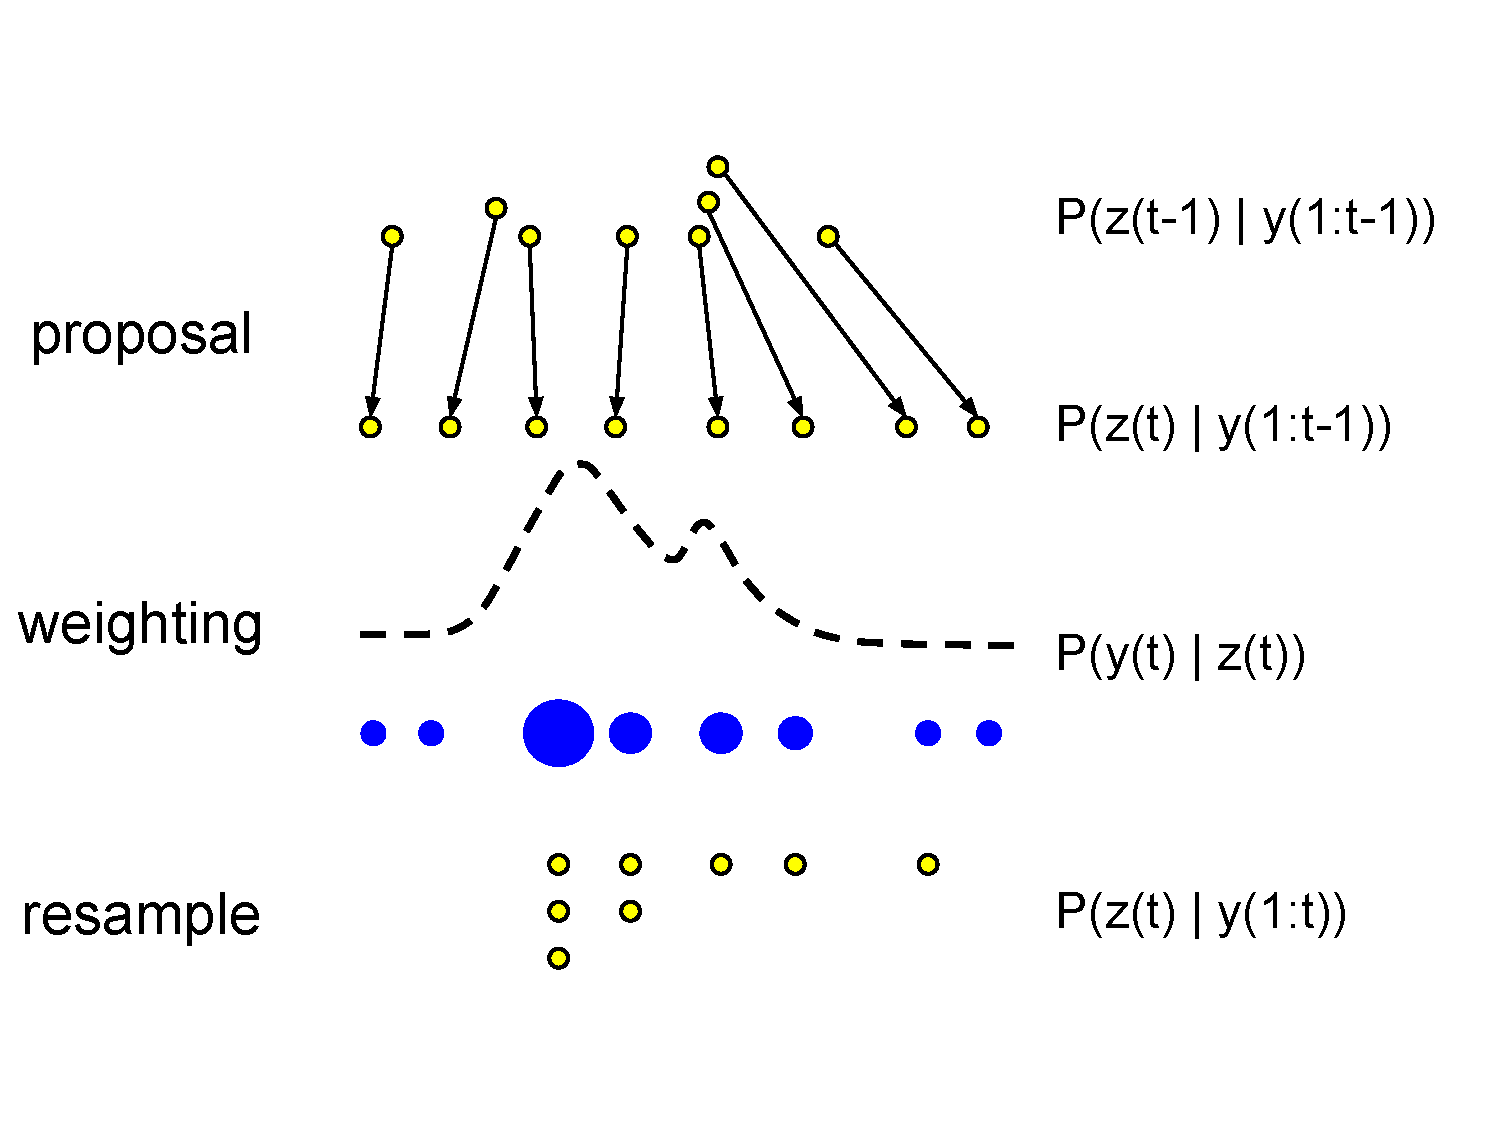
\includegraphics[width=0.4\textwidth]{pf}
\caption{Illustration of particle filtering.}
\end{figure}
\end{frame}

\begin{frame}{Particle filtering algorithm}
The basic algorithm is now very simple: for each old samples, propose an extension using $\bm{z}_t^s \sim q(\bm{z}_t|\bm{z}_{t-1}^s, \bm{y}_t)$, and give this new particle weight $w_t^s$.

\noindent\rule[-5pt]{\textwidth}{0.4pt}
{\footnotesize
\begin{tabbing}
    {\bf for} $s=1:S$ {\bf do}\\
    \qquad \= 1.\ Draw $\bm{z}_t^s \sim q(\bm{z}_t|\bm{z}_{t-1}^s, \bm{y}_t)$. \\
    \> 2.\ Compute weight $w_t^s \propto w_{t-1}^s\frac{p(\bm{y}_t|\bm{z}_t^s)p(\bm{z}_t^s |\bm{z}_{t-1}^s)}{q(\bm{z}_t^s |\bm{z}_{t-1}^s, \bm{y}_{t})}$.\\*[\smallskipamount]
    {\bf given} $x^k$, $\lambda^{k-1}$, and parameter $\beta \in (0,1)$. \\*[\smallskipamount]
    Normalize weights: ${\hat{w}}^s = \frac{w_t^s}{\sum_{s'}{w_t^s}'}$.\\
    Compute $\hat{S}_{\text{eff}} = \frac{1}{\sum_{s=1}^S}(w_t^s)^2$\\*[\smallskipamount]
    {\bf If} $\hat{S}_{\text{eff}}<S_{\text{min}}$ {\bf then}\\
    \qquad \= 1.\ Resample $S$ indcies $\pi\sim w_t$. \\
    \> 2.\ $\bm{z}_t = \bm{z}_t^{\pi}$. \\
    \> 3.\ $w_t^s = 1/S$. \\*[\smallskipamount]
    {\bf return} $p(z_{1:t}|\bm{y}_{1:t})$.
\end{tabbing}}
\noindent\rule[10pt]{\textwidth}{0.4pt}
\end{frame}

\end{document}
